\section{AMR} \label{Sec:AMR}

In general, the AMR input looks like:

\begin{Verbatim}[fontsize=\footnotesize]
  <AMR>
      <ICE>
        <do_Refluxing>        false    </do_Refluxing>
        <orderOfInterpolation>1         </orderOfInterpolation>
        <Refinement_Criteria_Thresholds>
          <Variable name = "press_CC" value = "1e6" matl = "0" />
        </Refinement_Criteria_Thresholds>
      </ICE>
      <MPM>
        <min_grid_level>-1</min_grid_level>
        <max_grid_level>-1</max_grid_level>
      </MPM>
      <useLockStep>true</useLockStep>
      <Regridder type="Tiled">
\end{Verbatim}

\begin{Verbatim}[fontsize=\footnotesize]
        <!--General Regridder Settings-->
        <max_levels>2</max_levels>
        <cell_refinement_ratio>    [[2,2,1]]</cell_refinement_ratio>
        <cell_stability_dilation>   [2,2,1]   </cell_stability_dilation>
        <cell_regrid_dilation>   [1,1,0]   </cell_regrid_dilation>
        <min_boundary_cells>       [1,1,0]   </min_boundary_cells>
\end{Verbatim}

\begin{Verbatim}[fontsize=\footnotesize]
        <!--Tiled Specific Settings-->
        <min_patch_size>  [[8,8,1]] </min_patch_size>
        <patches_per_level_per_proc>8</patches_per_level_per_proc>
      </Regridder>
    </AMR>

\end{Verbatim}

When running an ICE simulation, you must specify the following tags in the ICE section of your input deck.

\begin{itemize}
\item do\_refluxing - specifies whether or not to perform refluxing (true or false),
  which equalizes the face values of coarse/fine boundaries between
  levels.
\item orderOfInterpolation - specifies how many coarse cells to use
  when refining the coarse-fine interface (see below).
\item Refinement\_Criteria\_Thresholds section specifies the
  variables whose value will determine where to mark refinement flags,
  see below. Variables need only be specified on adaptive problems.
\item min\_grid\_level (optional) - coarsest level to run ICE on
  (default = 0).
\item max\_grid\_level (optional) - finest level to run ICE on (default
  = max-level -1).

\end{itemize}

If you run an MPM simulation, you must specify the MPM section, and
set min\_grid\_level and max\_grid\_level to the finest level of the
simulation, 0-based (i.e., if there are 2 levels, the level needs to
be set to 1). A shortcut to this is to set min- and max\_grid\_level to
-1.

\begin{itemize}
\item useLockStep - Some simulations require a lock step cycle (mpmice
  and implicit ice), as there has to be inter-level communication in
  the middle of a timestep. See ``W-cycle'' diagram below. Otherwise the
  time refinement ratio will be computed from the cell refinement
  ratio.
\end{itemize}


The presence of the Regridder section specifies you want to run an
adaptive problem.
\begin{itemize}
  \item type (optional) - sets the Regridder type. The options are
   ``Tiled'' (default), ``SingleLevel''.
 \item max\_levels - maximum number of levels to create in the grid.
 \item cell\_refinement\_ratio - How much to refine a cell in each
   dimension. This can be specified in a comma-separated list, with the dimensions in the default order [[x,y,z]].
    \item cell\_stability\_dilation - How much to pad the refinement flags
   in each dimension for stability reasons.  Reset on every timestep.
 \item cell\_regrid\_dilation - How much to pad the refinement flags in
   each dimension in order to reduce regridding frequency. If the refinement flags are still in the finest level due to large enough padding then regridding will not occur. Reset only when regridding occurs.
 \item min\_boundary\_cells - The minimum number of cells that needs to
   exist between one level's coarser level and its finer level (i.e.,
   between level 0 and 2).
\end{itemize}

When running a non adaptive problem. Adaptive regridding can be turned off by commenting out the regridding section.
\begin{itemize}
  \item min\_timestep\_interval - The minimum number of timesteps between each regrid. This will not force a regrid but after the set number of timesteps a regrid will be considered. Only used when adaptive regridding is turned off. min\_timestep\_interval $\leq$ cell\_stability\_dilation + 1
  \item max\_timestep\_interval - The maximum number of timesteps between each regrid.  This will not force a regrid.
 It tells the code it has been a set number of timesteps since the last regrid and it should look at if a regrid is needed. Used primarily when adaptive regridding is turned off.
\end{itemize}

Tiled Specific Settings
\begin{itemize}
\item min\_patch\_size - sets the minimum patch size created by the
  regridder per level. This size must divide evenly into the
  resolution and must be divisible by the cell refinement ratio.
\item patches\_per\_level\_per\_proc - sets the number of patches per
  level per processor that the load balancer attempts to achieve. If
  the number of patches is significantly more than the number
  specified the tiled regridder will increase the tile size by a
  factor of two in order to reduce the number of patches.
\end{itemize}

An example of a simple, 2-dimensional, tiled AMR problem can be found at \tt StandAlone/
inputs/MPMICE/advect\_2L\_MI.ups. \normalfont When the AMR input for this simulation matches the input at the beginning of this section (\ref{Sec:AMR}), we see the following:

\begin{figure}[H]
  \centering
  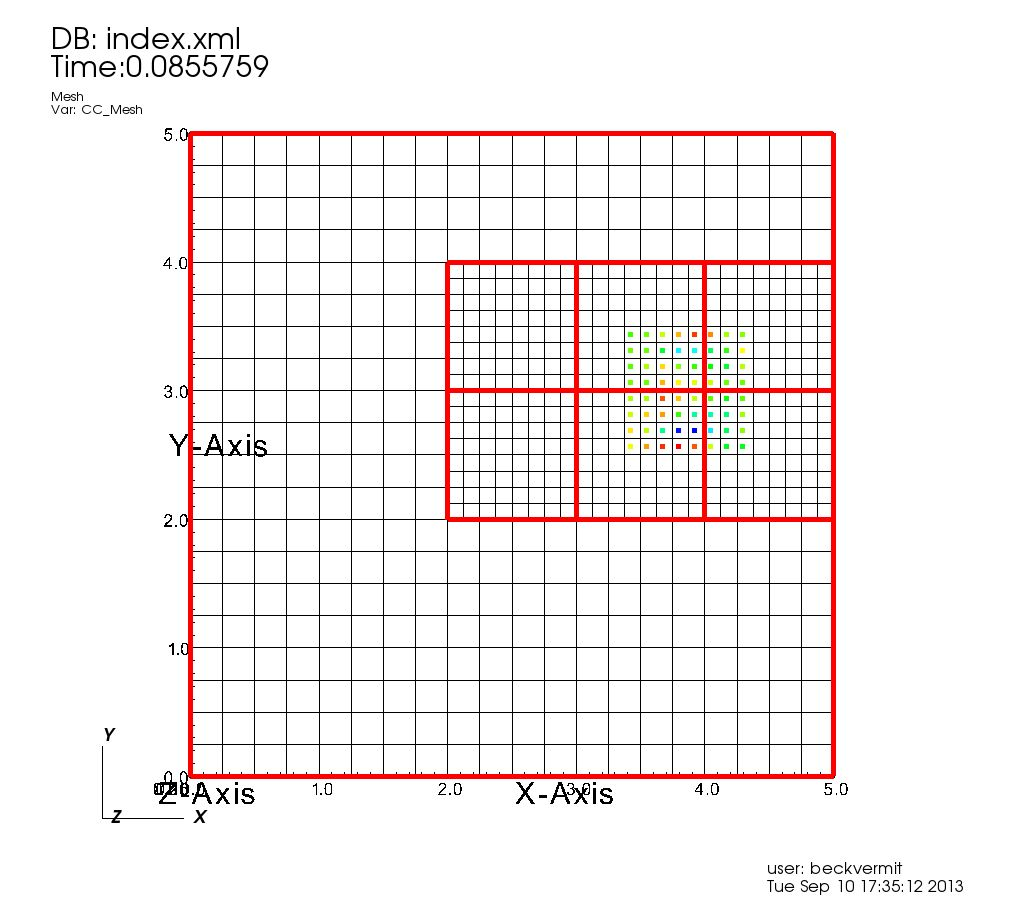
\includegraphics[trim=0cm 3cm 0cm 3cm, clip=true, width=1.\textwidth]{min-patch-size-8-8-1.jpeg}
  \caption{Advect\_2L\_MI with a minimum patch size of [8,8,1]}
  \label{fig:881}
\end{figure}

Here the black lines represent cells and the red lines represent patches with the box of multi-colored points being particles. As can be seen, there are 8 cells per patch in the x and y-direction and only one cell per patch in the z-direction (2D simulation). When we increase the minimum patch size to [20,20,1] we see:

\begin{figure}[H]
  \centering
  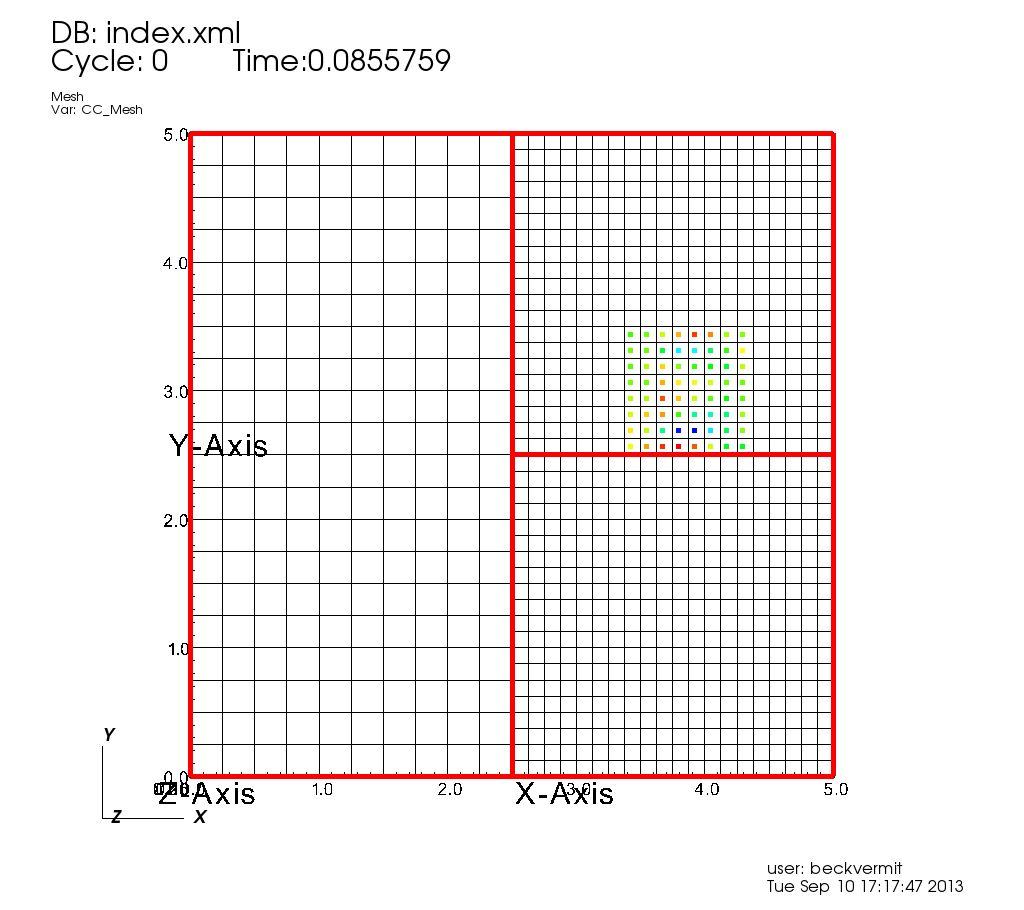
\includegraphics[trim=0cm 3cm 0cm 3cm, clip=true, width=1.\textwidth]{min_patch_size-20-20-1.jpeg}
  \caption{Advect\_2L\_MI with a minimum patch size of [20,20,1]}
  \label{}
\end{figure}

Note that now there are only 2 patches covering our finest level compared to the 6 patches covering our finest levels in figure \ref{fig:881}. This is because there is enough ``padding'' in between our refinement flags and differing levels to avoid setting up whole new patches at the most refined level. This option can be adjusted to increase or decrease the overall amount of regridding necessary with the cell\_regrid\_dilation flag.

When we decrease our minimum patch size to [4,4,1] we see:
\begin{figure}[H]
  \centering
  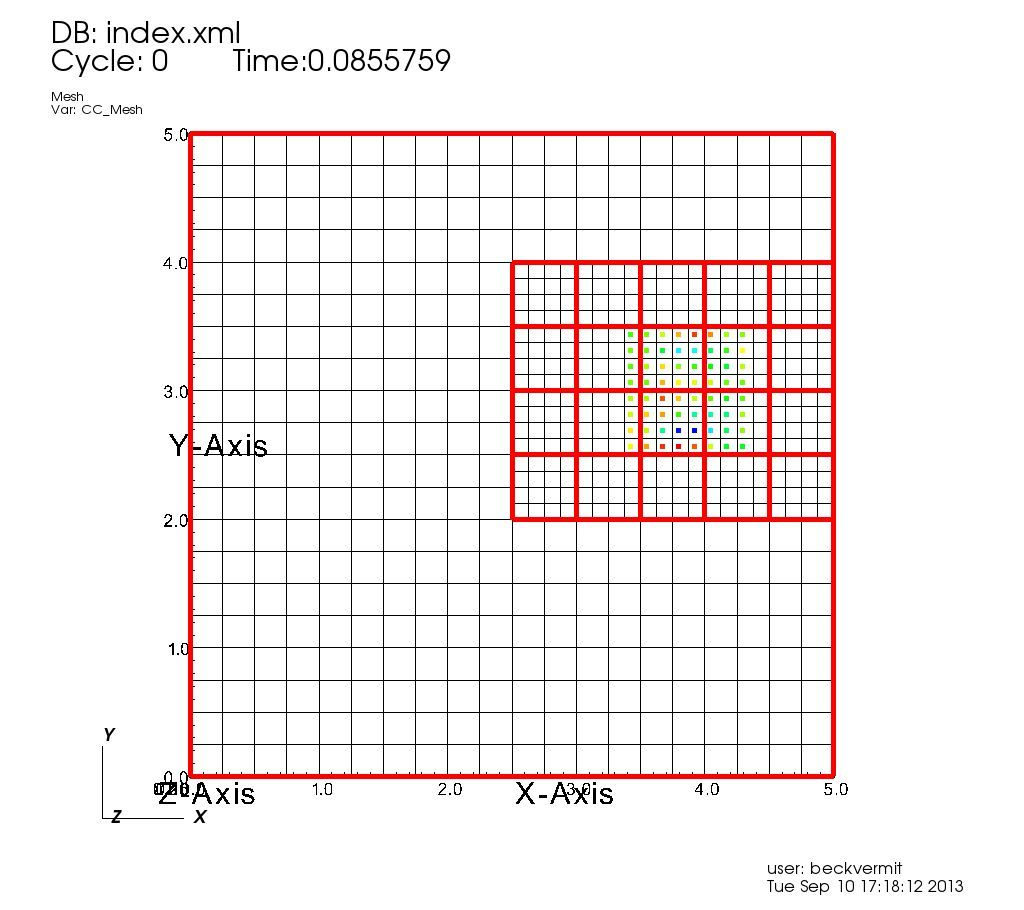
\includegraphics[trim=0cm 3cm 0cm 3cm, clip=true, width=1.\textwidth]{min_patch_size-4-4-1.jpeg}
  \caption{Advect\_2L\_MI with a minimum patch size of [4,4,1]}
  \label{fig:441}
\end{figure}

The best way to increase the ``padding'' of your simulation and therefore decrease the number of regrids required is to increase the cell\_stability\_dilation. Below we see the 2 dimensional example with a minimum patch size of [8,8,1], like figure \ref{fig:881}, but with a cell stability dilation of [10,10,1] rather than [2,2,1].

\begin{figure}[H]
  \centering
  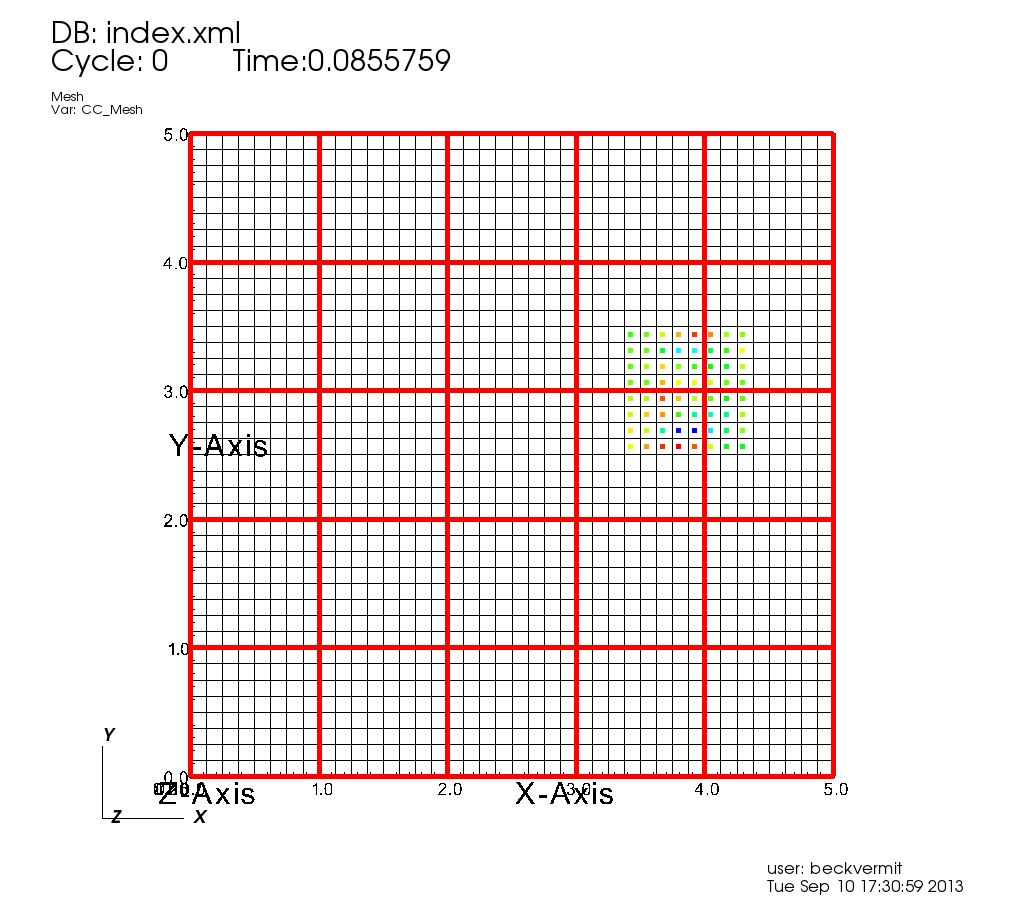
\includegraphics[trim=0cm 3cm 0cm 3cm, clip=true, width=1.\textwidth]{cell_stability_dialation-10-10-1.jpeg}
  \caption{Advect\_2L\_MI with a minimum patch size of [8,8,1] and a cell stability dilation of [10,10,1]}
  \label{fig:10101}
\end{figure}

There is a balance between cell stability dilation and computational time. If your domain is set up like figure \ref{fig:10101}, less computational time will be wasted regridding. However, it could be more economical to utilize some coarser levels in the areas that see little or no particles.


\subsection{AMR Grids}


There are two ways to run with mesh-refinement, either adaptive or
non-adaptive (static). Adaptive grids are created based on the
existence of refinement flags that are created during the
simulation. A regridder will analyze the whole domain, and, wherever there are
refinement flags, construct patches around them on a finer
level. See more on Regridding below.

\subsubsection{Regridding}


For an adaptive problem, specify the Regridder section in the input
file. The Tiled regridder works as follows:

Tiles sized according to the minimum patch size are laid across domain. Refinement flags are then used to determine which of
those tiles are in the patch set. If the number of tiles is more than
twice the target number of patches then the tile size is doubled in
the shortest dimension. If the number of tiles is less than the target
number of patches then the tile size is halved in the longest
dimension. The tile size will never get smaller than the minimum
specified tile size. This regridder produces regular patch sets that
are easy to load balance. After patches are added, data is stored on them. Then data will be
initialized for those new patches, and in the next timestep, those
patches will be included in the regridding process.

A constraint of the Regridder is that any two patches that share a boundary must be within one level of each other. See (E) and (F) below.

%At initialization time, the regridder can be executed and then the
%problem reinitialized so the problem can be initialized with all
%5max\_levels of refinement.

\begin{figure}[H]
  \centering
  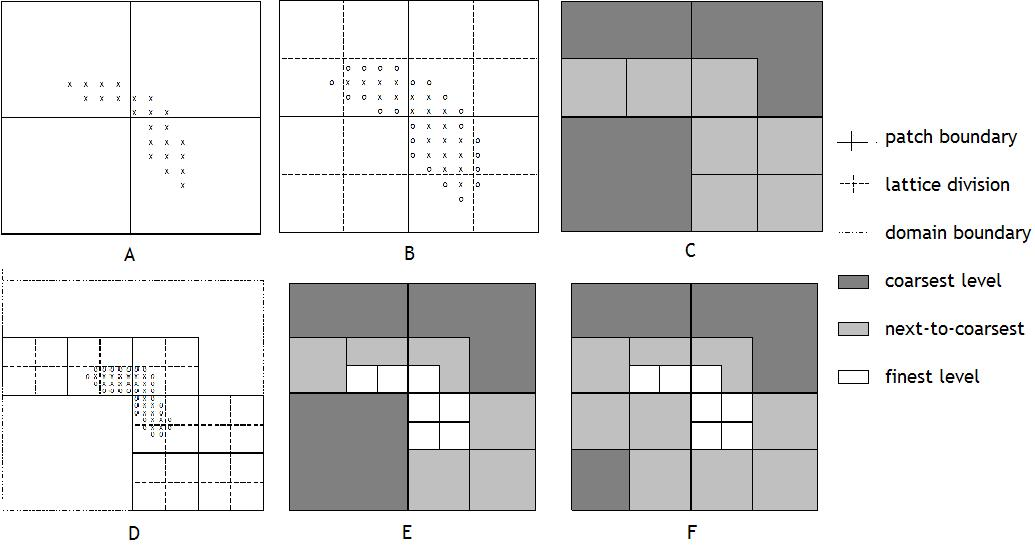
\includegraphics[width=1.\textwidth]{AMR-Regridding.jpg}
  \caption{}
  \label{}
\end{figure}

In the diagram above, image (A) show 4 coarse patches with some marked
error flags. (B) Shows the subpatches for the next level and has the
error flags dilated. (C) Shows the coarse level together with the fine
level you end up with.

(D) During the next regrid, the next level can create error flags as
well. These are some example error flags that are dilated, with the
subpatches for the next level. (E) shows the resulting level with the
other levels. However there are some patch boundaries that span more
than one level. So in (F) we must expand out the middle level to
compensate.

Note that if you define multiple levels in the input file, all but
the coarsest level will be recycled, and levels will be added where
the Regridder wants to put them.

\subsubsection{Static Grids}

Static grids can be defined by simply not including a Regridder
section in the input file. See the multiple level example in
Grid~\ref{Sec:Grid}.

\subsubsection{Ideal Patch Configuration for Good Scaling}
The patch configuration on multiple levels has been shown to greatly
effect the scalability and mean time per time step.
Here are some guidelines to follow when trying to get good scaling with multilevel AMR.
This example is for a 3 Level simulation.
\begin{itemize}
\item On Level 0 and 1 $\frac{\# cells}{patch} = 8$ \\	
	i.e. min\_patch\_size [8,8,8]
\item On finer levels (level 2)
\begin{itemize}
	\item min\_patch\_size MUST be greater than or equal to 8,8,8!! This is very important!
	\item $\frac{\# cores}{2} $ $\leq$ $\#$ patches on the finest level $\leq$ $\#$ cores
	\item The min\_patch\_size on L-2 must be divisible by the min\_patch\_size on L-1
\end{itemize}
\end{itemize}

\subsection{AMR Cycle}

Whether working with an adaptive or a static grid, AMR problems follow
the same cycle.

In short, there are 3 main AMR operations
\begin{itemize}

\item Coarsen - This occurs after each execution of a finer level, if
  the time of the finer level lines up with the time of the coarser
  level (see the ``W-cycle'' diagram). Its data are coarsened to the
  coarser level so that the coarse level has a representation of the
  data at the finest resolution. Also as part of this operation is the
  ``reflux'' operations, which to makes the fluxes across the face of
  the coarse-fine boundary consistent across levels.
\item Refine the coarse-fine interface - This occurs after the
  execution of each level and after an associated coarsen (if
  applicable). The cells of the boundary of the finer level are
  interpolated with the nearest cells on the coarser level (so the
  finer level stays in sync with the coarser levels).
\item Refine - This occurs for new patches created by the regrid
  operation. Variables that are necessary will be created on those
  patches by interpolation from the coarser level.
\end{itemize}

After an entire cycle, then we check to see if we need to regrid. If the flags haven't changed such that patches would form, the grid will remain the same.

In short, these diagrams may be useful:

``W-cycle'' (time refinement ratio of 2)

\begin{figure}[h]
  \centering
  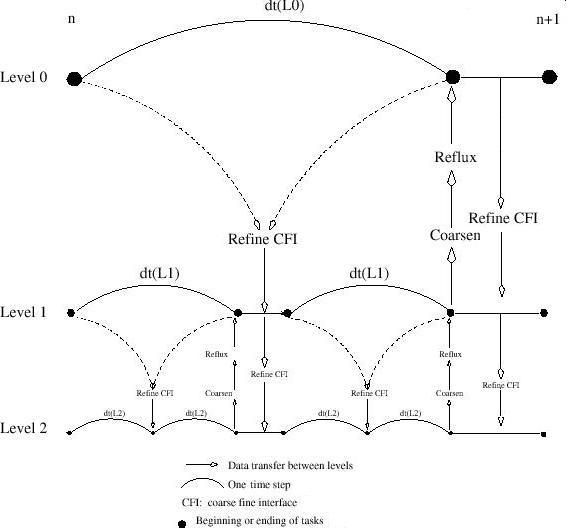
\includegraphics[width=.75\textwidth]{AMR-Cycle-W.jpg}
  \caption{}
  \label{}
\end{figure}

``Lockstep cycle''

\begin{figure}[h]
  \centering
  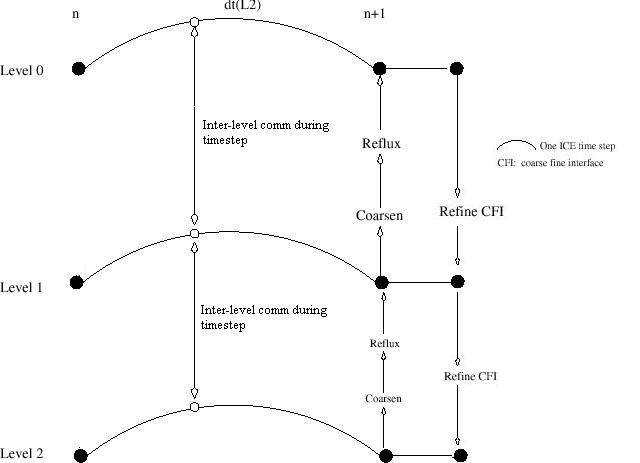
\includegraphics[width=.75\textwidth]{AMR-Cycle-Lock.jpg}
  \caption{}
  \label{}
\end{figure}
